

\section{Results}
This chapter will focus on providing visual representations of the findings from the experiment. These findings will be described in detail to further be used to evaluate the hypothesis in the discussion section of the report. 


\subsection{Relationship between training iterations and loss}
\begin{figure}[h]
   \centering
   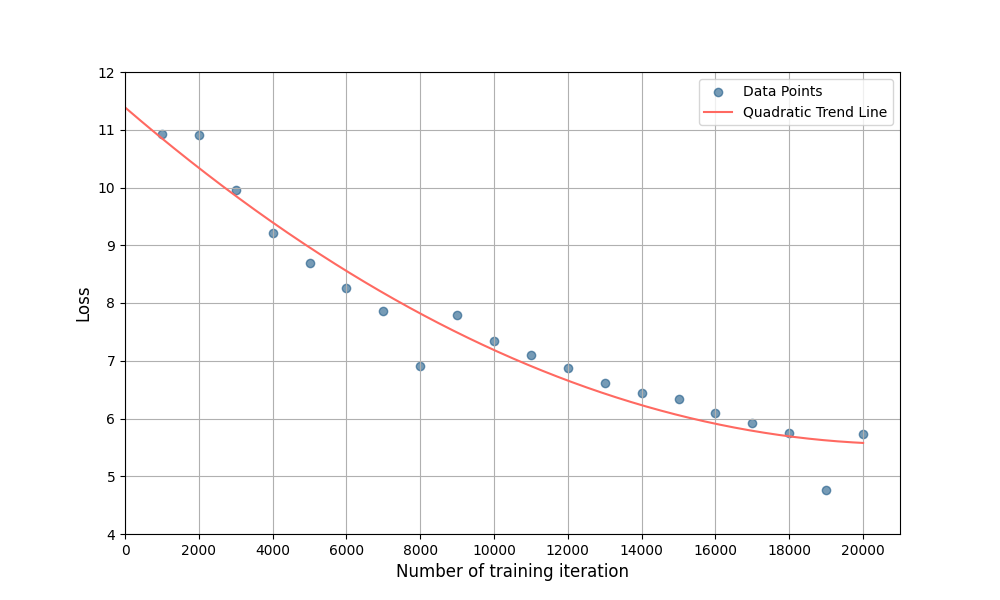
\includegraphics[width=0.9\textwidth]{../Data/loss_by_iteration_plot.png}
   \caption{Quadratic Trend Analysis of Loss Reduction Over 20,000 Training Iterations}
   \label{fig:loss-vs-training-iterations}
\end{figure}
The data illustrated in Fig.\ref{fig:loss-vs-training-iterations} displays the relationship between the the loss of the object detection model over the 20,000 training iterations of the machine learning algorithms. It can be seen that during the initial stages of the experiment, a sharp decline in the loss can be viewed. This demonstrates the initial learning phase of the program. However, with an increased number of training iterations, the rate of the loss decreasing steadily slows down as it approaches its optimal state. \\

The quadratic trendline graphed in Fig.\ref{fig:loss-vs-training-iterations}  displays the model approaching a state of convergence, as the training iteration count increases and loss decreases. Furthermore, the trendline expresses the non-linear relationship between training iterations and the loss of the model. \\


\subsection{Relationship between training iterations and accuracy}
- line graph of accuracy against interation
- precntage development of accuracy    against interation


\subsection{}
- box plot per iteration 



